%************************************************
\chapter{Appendix}\label{ch:appendix}
%************************************************
\begin{table}[ht]
		    \myfloatalign
		    \begin{tabularx}{\textwidth}{rrr} \toprule
		        \tableheadline{Mels} & \tableheadline{Hz}
		        & \tableheadline{Filterbank} \\ \midrule
		        % Phantoms take care of right-alignment (works iff monospaced digits)
		        0    & 0\phantom{.0} & 0 \\
		        105  & 68.5   & 2 \\
 		        210  & 143.7  & 4 \\
 		        315  & 226.2  & 7 \\
		        420  & 316.8  & 10 \\
		        525  & 416.3  & 13 \\
		        630  & 525.5  & 16 \\
		        735  & 645.4  & 20 \\
		        840  & 777\phantom{.0} & 24 \\
		        945  & 921.5  & 29 \\
		        1050 & 1080.1 & 34 \\
		        1155 & 1254.4 & 40 \\
		        1260 & 1445.4 & 46 \\
		        1365 & 1655.3 & 53 \\
		        1470 & 1885.7 & 60 \\
		        1575 & 2138.6 & 68 \\
		        1680 & 2416.3 & 77 \\
		        1785 & 2721.2 & 87 \\
		        1890 & 3055.9 & 97 \\
		        1995 & 3423.3 & 109 \\
		        2100 & 3826.7 & 122 \\
		        2205 & 4269.5 & 136 \\
		        2310 & 4755.7 & 152 \\
		        2415 & 5289.4 & 169 \\
		        2520 & 5875.3 & 188 \\
		        2625 & 6518.6 & 209 \\
		        2730 & 7224.8 & 231 \\
		        2835 & 8000\phantom{.0} & 256 \\
				\bottomrule
		    \end{tabularx}
		    \caption[Filterbanks]{Conversion table between linearly spaced Mels and their corresponding frequencies and filterbank boundaries.}  \label{tab:mels}
		\end{table}


\begin{figure}[ht]
    \centering
    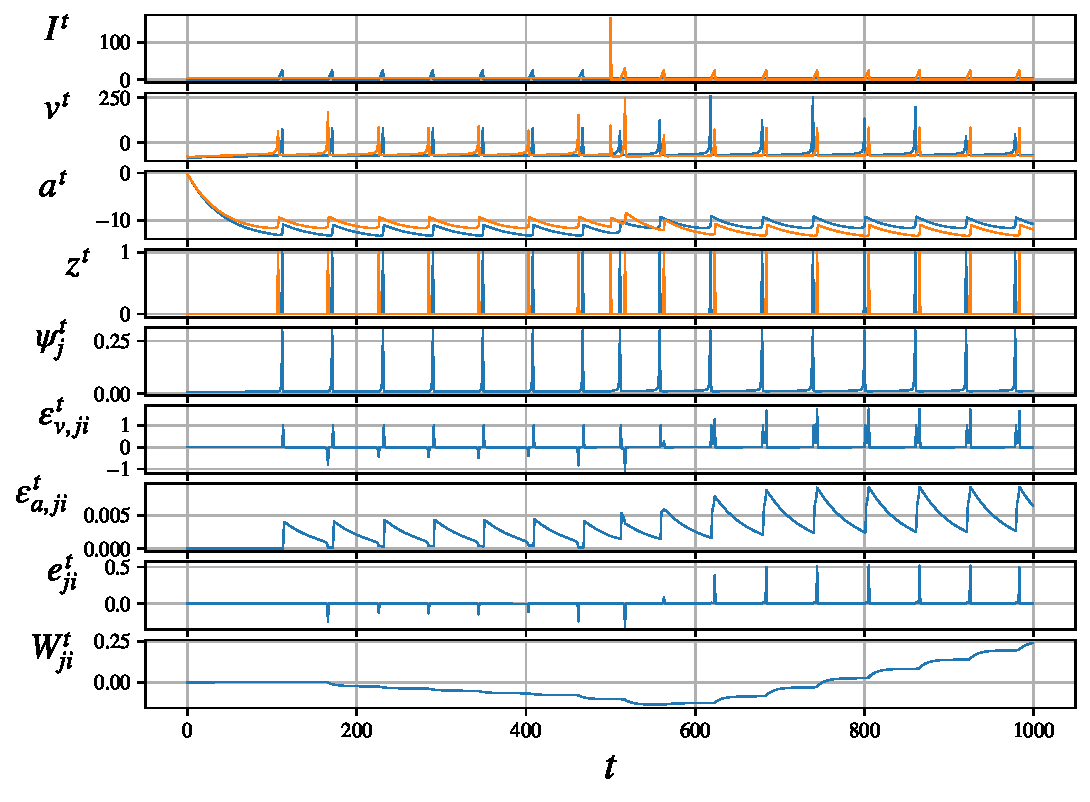
\includegraphics[width=\linewidth]{gfx/demo_izh}
    \label{fig:demo_izh}
    \caption{A single-synapse demo of the uncorrected Izhikevich neuron. Note that $\epsilon^t_{ji, v}$ takes on extreme values and that the eligibility vector flips sign at any pair of spikes.}
\end{figure}
